%%%%%%%%%%%%%%%%%%%%%%%%%%%%%%%%%%%%%%%%%%%%%%%%%%%%%%%%%%%%%%%%%%%%%%%%
% Preamble
%%%%%%%%%%%%%%%%%%%%%%%%%%%%%%%%%%%%%%%%%%%%%%%%%%%%%%%%%%%%%%%%%%%%%%%%
\documentclass[11pt]{article}
%
% Packages and other includes
% Pagination
\usepackage[letterpaper, margin=1in]{geometry}
\usepackage{emptypage}
%
% Fonts
\usepackage[T1]{fontenc} % best for Western European languages
\usepackage{lmodern} % Latin Modern instead of CM
\usepackage{textcomp} % required to get special symbols
%
% Math
\usepackage{amsmath, amssymb}
\usepackage{braket}
%
% Graphics, floats, tables
\usepackage{graphicx, color, float, array}
%
% Hyperlinks
\usepackage{hyperref}
%
%
% Definitions and settings
% Paragraph indent and spacing
\setlength{\parskip}{0.4\baselineskip}
\setlength{\parindent}{0in}
%
%
% Title, authors, date
\title{\textbf{Worksheet 2}}
\date{\vspace{-2em}January 11, 2022}
%
%
%%%%%%%%%%%%%%%%%%%%%%%%%%%%%%%%%%%%%%%%%%%%%%%%%%%%%%%%%%%%%%%%%%%%%%%%
% Main document
%%%%%%%%%%%%%%%%%%%%%%%%%%%%%%%%%%%%%%%%%%%%%%%%%%%%%%%%%%%%%%%%%%%%%%%%
%

\begin{document}

\maketitle

Weekly homework assignments are posted approximately one week prior to the
due date. Collaborations are encouraged and students must report all collaborators
in writing on each assignment. All external sources (websites, books) must be
properly cited. Additional problems are listed at the end of each assignment.
This week's assignment is due \textit{Tuesday, Jan 18th at 10:00am.}

\textbf{Ideal Gas Law}

1. (2 pts) What\ is the density (in g/L) of chloroform, CHCl$_3$, vapor at
$2.00\times 10^2\text{Torr}$ and $298\text{K}$.

\vspace{1in}

2. (2 pts) A compound used in the manufacture of Saran is $24.7\%$ C, $2.1\%$ H, and
$73.2\%$ Cl by mass. The storage of $3.557\text{g}$ of the gaseous compound in
a $755$-mL vessel at $0^\circ\text{C}$ results in a pressure of $1.10\text{atm}$.
What is the molecular formula of the compound?

% C2H2Cl2

\vspace{1in}

3. (2 pts) A vessel of volume $22.4\text{L}$ contains $2.0$ mol H$_2$(g) and $1.0$ mol
N$_2$(g) at $273.15\text{K}$. Calculate the partial pressures and the total pressure.

\vspace{1in}

\textbf{Real Gases}

4. (2 pts) The pressure of a sample of hydrogen fluoride is lower than expected and, as the
temperature is increased, rises more quickly than the ideal gas law predicts.
Suggest an explanation.

\vspace{1in}

\textbf{First Law of Thermodynamics}

5. (3 pts) Below there are pictures showing a molecular view of a system
undergoing a change. In each case, predict the signs of $q$ and $w$ for
 each process. Explain what is happening to the system.

\begin{center}
  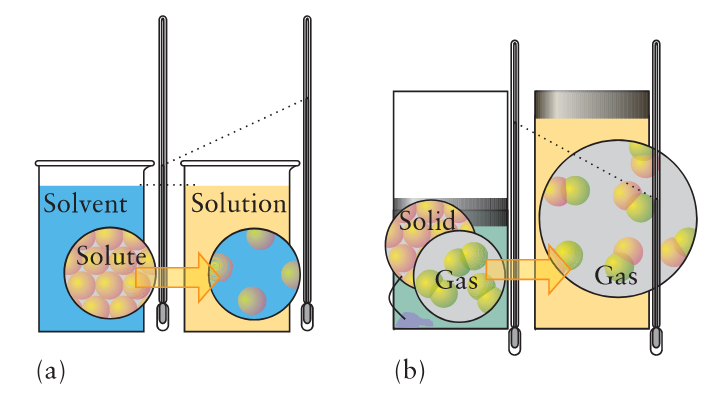
\includegraphics[scale=0.35]{phase_change.png}
\end{center}

\vspace{1in}

6. (4 pts) Calculate the work for each of the following processes beginning with a gas
sample in a piston assembly with $T=305\text{K}$, $P=1.79\text{atm}$, and
$V=52.9\text{L}$ by two different pathways.

(a) Isothermal, reversible expansion to a final volume of $6.52\text{L}$.

(b) Irreversible expansion against a constant external pressure of $1.00\text{atm}$
to a final volume of $6.52\text{L}$.

\vspace{1.5in}


\vfill
\textbf{Optional Additional Problems:} Ch. 9 - odd problems 

\end{document}
